\documentclass{article}

\usepackage[utf8x]{inputenc}
\usepackage[spanish]{babel}
\usepackage[margin=3cm]{geometry}
\usepackage{amsmath}
\usepackage{amssymb}
\usepackage{graphicx}
\usepackage{algorithm}
\usepackage{algorithmic}

\linespread{1.2}

\title{Computación Concurrente \\ \Large{Tarea Exámen 1}}
\author{
  Diego Goméz Montesinos
  \and
  José Emiliano Cabrera Blancas
  }
\date{4 marzo 2014}
\begin{document}
\maketitle
\begin{enumerate}
  
\item{
    \textsl{
      En clase hemos visto mapas portadores y mapas simpliciales. Sea $\Xi$ un
      mapa portardor y sea $\delta$ un mapa simplicial que preserva estructura,
      demuestra que si la composición $\delta \circ \Xi$ es un mapa portador, 
      entonces $\Xi \circ \delta$ es un mapa portador.\\
    }
    
    Por demostrar:\\
    Si la composición $\delta \circ \Xi$ es un mapeo portador $\Rightarrow$ 
    $\Xi \circ \delta$ es un mapeo portador.
    
    Demostración:\\
    Primero hacemos una observación, sea $v \in G$, por hipótesis la siguiente 
    proposición se cumple: $\delta(v) \in G$ y $\Xi(v) \in G$.\\
    Dado que $\Xi$ es un mapeo portador, sabemos que si $\tau \in G$ y 
    $\sigma \in G$ $\Rightarrow$ $\Xi(\tau)$ $\subseteq$ $\Xi(\sigma)$(es monótono).\\
    Por lo que si $\delta(\Xi(G))$ es un mapeo portador, entonces $\delta(u)$ es un
    mapeo portador con $u \in \Xi(G)$, dicho de otra forma, $\tau' \in \Xi(G)$ y 
    $\sigma' \in \Xi(G)$, donde $\tau'$ $\subseteq$ $\sigma'$ $\Rightarrow$ $\delta(\tau') 
    \subseteq \delta(\sigma')$.\\
    Como $\Xi(G) = G$, entonces por lo anterior $\delta$ es un mapeo portador.
    Lo que indica que $forall$ $v$,$u$ $\in G$, tal que $v \subseteq u$ $Rightarrow$ 
    $\delta(v)$ $\subseteq$ $\delta(u)$, y dado que $\Xi$ es un mapeo portador, entonces
    se cumple que $\Xi(\delta(v))$ $subseteq$ $\Xi(\delta(u))$, por lo tanto la composición
    $\Xi \circ \delta$ es un mapeo portador. $_\square$\\
        
  }
  
\item{
    \textsl{ 
      Diseña un algoritmo (secuencial) que dada una tarea $T = (\mathcal{I},\mathcal{O},\Delta)$
      conteste si tiene o no solución en el modelo iterado wait-free visto en clase, y si la tiene,
      conteste en a lo más cuantas capas. Analiza su correctez y complejidad (como función del tamaño
      de la entrada), suponiendo que para cada vértice $v$ de $\mathcal{I},\Delta(v)$ consiste de 
      un conjunto de a lo más $k$ vértices, para una constante k.
    }

    \textbf{SOLUCIÓN}\\
    Primero veamos el algoritmo verificador.\\
    En clase vimos el Teorema Principal para tareas de dos procesos: Dada una tarea $(\mathcal{I},\mathcal{O},\Delta)$
    tiene solución en el modelo iterado por capas si y solo si existe un mapeo portador conexo
    $\Phi: \mathcal{I} \rightarrow 2^{\mathcal{O}}$, portado por $\Delta$.\\
    Dado que el modelo iterado wait-free es un subconjunto del modelo iterado por capas, entonces, podemos
    aplicar el Teorema y decir que la tarea $T$ tiene solución si existe un mapeo portador conexo $\Phi$, portado por $\Delta$.\\
    Entonces el algoritmo tendría que verificar si existe o no tal mapeo portador conexo; ahora, dado que el mapeo portador
    $\Phi$ debe ser conexo, entonces debe ocurrir que $\forall\sigma\in\mathcal{I}$, $\Phi(\sigma)$ es una
    gráfica conexa. Pero como $\Phi$ es portado por $\Delta$, entonces tendríamos que ver que $\Delta$ fuera un mapeo portador
    conexo, ya que de lo contrario $\Phi$ no sería conexo.\\
    Entonces, la idea del algoritmo será recorrer $I$, e ir checando que $\Delta$, sea un mapeo portador conexo.
    Además llevaremos un contador de aristas, para ver cual es el camino más largo y en base a eso decir cuantas capas
    son necesarios para resolverlo.\\
    Dada la definición de mapeo portador conexo, el algoritmo quedaría de la siguiente manera:\\
    
    \begin{algorithmic}
    \STATE $m \leftarrow 0$ \COMMENT{En esta variable se guardarán la longitud del camino más grande (maximo).}
    \STATE $k \leftarrow 0$ \COMMENT{En esta variable se guardarán la longitud del camino actual.}
    \FORALL{arista $e\in\mathcal{I}$ \COMMENT{Esto se puede hacer con BFS ó DFS, empezando con una arista arbitraria}}
    \STATE $e \leftarrow $ arista actual
    \STATE $u \leftarrow $ un extremo de $e$
    \STATE $v \leftarrow $ el otro extremo de $e$
    \STATE $esConexo \leftarrow False$
    \FORALL{arista $e'\in\Delta(e)$ \COMMENT{Esto se puede hacer con BFS ó DFS, empezando con una arista adyacente a $\Delta(u)$}}
    \STATE $e' \leftarrow $ arista actual
    \IF{$e' \in \Delta(e)$}
    \STATE $u' \leftarrow $ un extremo de $e'$
    \STATE $v' \leftarrow $ el otro extremo de $e'$
    \IF{$u' == \Delta(v) \wedge v' == \Delta(v) $}
    \STATE $esConexo \leftarrow True$
    \ENDIF
    \STATE $k \leftarrow k + 1$
    \ENDIF
    \ENDFOR
    \IF{$!esConexo$}
    \RETURN $False$
    \ENDIF
    \STATE $m \leftarrow max(k, m)$
    \ENDFOR
    \RETURN $\lceil log_{3} m \rceil$
    \end{algorithmic}

    Dado que DFS y BFS son de complejidad $O(\mathcal{I}) = O(|V| + |E|)$, y suponemos que cada vértice $v$ de $\mathcal{I},\Delta(v)$
    consiste de un conjunto de a lo más $k$ vértices, para una constante k; entonces la complejidad del algoritmo es de
    $O((|V| + |E|) k)$.\\
    El algoritmo es correcto, ya que tanto $\mathcal{I}$, como $\mathcal{O}$ son finitas, es decir, ambos recorridos terminarán; además
    cumplirá con descubrir si algún $\Delta(e)$ no es conexo, y con esto ver si $\Delta$ es un mapeo portador conexo. Note que, por
    hacer el recorrido BFS o DFS nos vamos tomando aristas adyacentes, verificando de igual manera que si $v\subseteq\sigma\cap\tau$ entonces
    $\Delta(v)\subseteq\Delta(\sigma)\cap\Delta(\tau)$.
  }

\item {
    \textsl{
      En el modelo anónimo iterado para $n$ procesos, $n ≥ 1$, con $L = 1$ iteración, definir
      cuales son las posibles vistas de los procesos en una ejecución, cuyos valores de entrada
      son $S$. Es decir, para cada $x \in S$, al menos un proceso empieza con $x$. (pista: si el
      conjunto de entradas en la ejecución es un conjunto $S$, la vista de un proceso es un 
      subconjunto de $S$, y las vistas $S_1,S_2,...,S_k$ están en la misma ejecución si y solo si
      todas son subconjuntos de $S$, y se pueden ordenar de forma que cada una este contenida o
      sea igual a la siguiente).
    }

    \textbf{SOLUCIÓN}\\
    Primero veamos los casos sencillos. Supongamos que $S = \{S_{0}, S_{1}\}$, el complejo de entrada
    quedaría:\\
    \begin{center}
      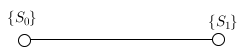
\includegraphics[scale=0.5]{input.png}
      \\\tiny{Complejo de entrada anónimo con $|S| = 2$.}
    \end{center}
    Ahora, después de una ronda de comunicación, este complejo queda de la siguiente manera:\\
    \begin{center}
      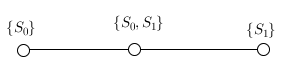
\includegraphics[scale=0.5]{input_1.png}
      \\\tiny{Complejo después de una ronda de comunicación con $|S| = 2$.}
    \end{center}
    El vértice $\{S_{0}\}$, representa a todos los procesos que tienen vista $\{S_{0}\}$ (análogo para $\{S_{1}\}$),
    y la arista $(\{S_{0}\}, \{S_{0},S_{1}\})$, representa la ejecución donde al menos un proceso tiene vista
    $\{S_{0}\}$, y al menos un proceso tiene vista $\{S_{0}, S_{1}\}$.
    Note que se cumple que las vistas están contenidas en $S$, $\{S_{0}\} \subseteq S$ y $\{S_{0},S_{1}\} \subseteq S$; y se pueden
    ordenar por conjunción: $\{S_{0}\} \subseteq \{S_{0},S_{1}\}$.\\
    Ahora veamos que pasa con $S = \{S_{0}, S_{1}, S_{2}\}$.\\
    \begin{center}
      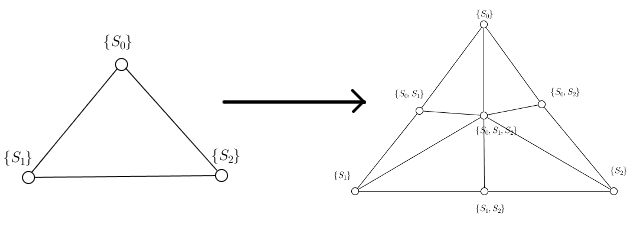
\includegraphics[scale=0.5]{input_2.png}
      \\\tiny{Con $|S| = 3$.}
    \end{center}
    Podemos ver que se cumplen las propiedades que son subconjuntos de $S$, y que se pueden ordenar por contención.\\
    Ahora daremos la generalización: si $|S| = k$ para alguna $k$ tal que $n ≥ k ≥ 1$; entonces el complejo de entrada
    será un simplejo de dimensión $|S| - 1$, que está formado por simplejos de dimensión $d = 0, 1, ..., k-1$. En la primera
    ronda de comunicación, cada uno de estos simplejos se subdividirán y el vértice central(simplejo de dimensión $d = 0$) tendrá
    vista de cardinalidad $d + 1$. Después todos los vértices se unirán al vértice central.\\
    Observe como esto se cumple en el ejemplo con $|S| = 3$.\\
    Dado que los simplejos se van subvididiendo y las vistas de sus vértices centrales tienen vista con cardinalidad $d + 1$, entonces
    se puede ordenar por contención.
  }
  
\item{
    \textsl{
      Demuestra que un modelo anónimo y un modelo cromático tienen el mismo poder de cómputo, es
      decir, todas las tareas anónimas, $\langle \mathcal{I},\mathcal{O},\Delta \rangle$ tal que
      $\mathcal{I}$ y $\mathcal{O}$ no tiene colores, que se pueden resolver en un modelo anónimo
      también las puede resolver un modelo cromático.\\
      Considera modelos para dos procesos, iterado y wait-free.\\
    }

    La idea de la demostración es dada la tarea $T$ en el modelo anónimo, debemos de dar una serie de mapeos
    que conviertan la tare $T$ a una tare $T'$ en el modelo cromático y al final contruir una $\delta'$ que resuelva
    la tarea $T'$

    Demostración:\\
    Sea $T$ una tarea definida por $\langle$ $\mathcal{I},\mathcal{O},\Delta$ $\rangle$ con $\mathcal{I}$
    y $\mathcal{O}$ gráficas anónimas. Por hipótesis decimos que existe una $\delta$ un mapeo portador
    tal que resuelve la tarea dada.
    Para esto debemos dar la tarea $T'$ definida por $\langle$ $\mathcal{I}',\mathcal{O}',\Delta'$ $\rangle$
    tal que es la representación de la tarea $T$ en el modelo cromático.\\
    Para esto vamos a definir $\Phi$ $:$ $\mathcal{I}$ $\xrightarrow{}$ $\mathcal{I}'$ de la siguiente forma:\\

    \begin{itemize}
      \item{
          $\Phi(v_i) = (v_{ia},v_{ib})$
        }
         \item{
             $\Phi((v_i,v_j)) = (v_{ia},v_{jb}), (v_{ib},v_{ja})$
        }
    \end{itemize}

    Dicho de otra forma, cuando $\Phi$ recibe un vértice con etiqueta i, este lo mapea a una arista con dos vértices
    con etiquetas i y con color distinto entre si(a y b son los colores), cuando $\Phi$ recibe una arista, entonces la 
    mapea a dos aristas con vertices con etiquetas iguales, agregando color a los vértices.

    \begin{center}
      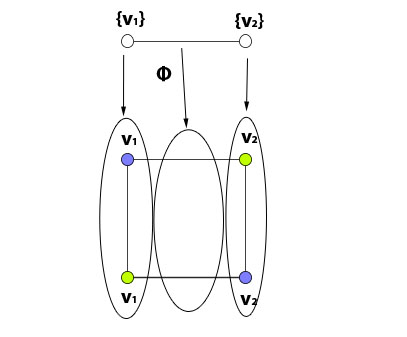
\includegraphics[scale=0.6]{5_input.jpg}
      \\Ejemplo de mapeo de una gráfica anónima con vertices $v_1$ y $v_2$ a una gráfica cromática.
    \end{center}

    Es fácil definir una función $\Gamma$ definida de igual forma que $\Phi$(las mismas reglas para vertices y para aristas),
    pero con dominio e imagen
    $\Gamma$ $:$ $\mathcal{O}$ $\xrightarrow{}$ $\mathcal{O}'$\\
    Por úlitmo definimos el mapeo portador $\Delta'_i$ = $\Phi'_i \circ \Delta_i$ donde $\Phi'_i$ es una función que apartir de un vértice
    anónimo con la etiqueta correspondiente a la ronda $i$ genera una subgráfica cromática con todas las posibilades del conjunto de
    vértices que representa el vértice anónimo, y si recibe una arista, entonces mapea la arista a una subgráfica cromática con todas 
    las posibilidades del conjunto de vértices que representa el vértice anónimo.

    \begin{center}
      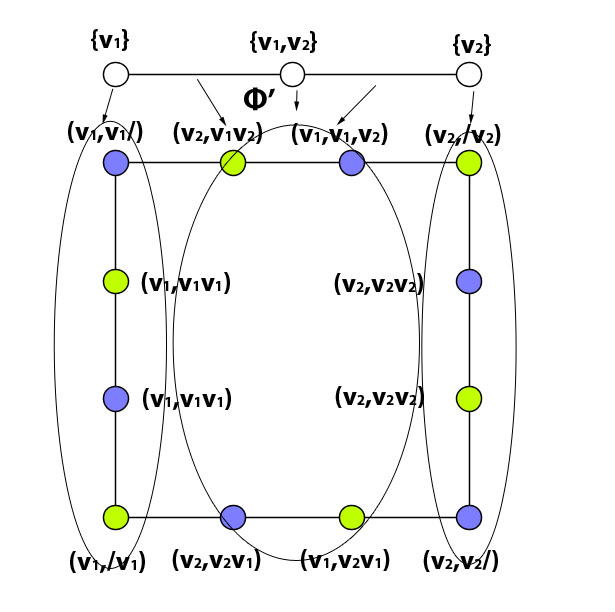
\includegraphics[scale=0.4]{5_Delta.jpg}
      \\Ejemplo de la función $\Phi'$ de la primera ronda de la gráfica anónima del ejemplo anterior con vertices $v_1$ y $v_2$ a una gráfica cromática.
    \end{center}

    Por último falta definir un mapeo $\delta'$ que resuelve la $T'$ que previamente contruimos, ésta la contruimos como 
    $\delta'(v_{ic}) = \delta(v_{i}) +  c$, donde $c$ es el color del vértice y la operación $+ c$, es concatenarle el color que pierde
    del mapeo $\delta$.\\
    Es fácil ver que el mapeo $\delta'$ es un mapeo portador, por que ''conserva'' la monotocidad que aporta $\delta$, esto es:
    si $\sigma$ y $ \tau \in \Delta'(\mathcal{I}')$, tal que $\tau \subseteq \sigma$ entonces $\delta'(\tau) \subseteq \delta'(\sigma)$.\\

    Por lo tanto $\delta'$ resuelve la tarea $T'$. Por lo tanto el modelo cromático tiene el mismo poder de compúto que el modelo anónimo. 
  }
\end{enumerate}
\end{document}